\section{Introduction}
% task introduction
% jiac: I'm lazy and some of the content in this paragraph is almost the same as that in 1st paragraph in the technical report. Would you please slightly change the presentation of these sentences? Especially the 1st sentence. 
% it would be better to also ps different view images of the boston dataset in th figure~\ref{fig:library}
With the popularity of smartphones equipped with high quality cameras, events around the world can be quickly captured by videos and rapidly shared via social media.
When an event happens, different videos capture the same event at different positions from different perspectives.
For example, videos from surveillance cameras usually cover the event from a fixed location from 45 degree angle; 
videos from television reporters usually record the event in a rather professional perspective (helicopter view or first person view) at major locations; 
the videos from passersby usually capture event from a personal perspective at side locations that are often not covered by the news reporters.
On the one hand, knowing where is the video content is the basic and essential element behind various event analysis tasks such as person tracking and scene reconstruction. 
On the other hand, unlike EXIF meta-data in images, most of the videos shared online don't come with GPS information together. 

% task definition
In this paper, we study the problem of automatic event video localization. 
The input of event video localization is the query, event video, and the database, environment images with gps information, which could be street view images if the event video is taken on the ground or satelite images if the event video involves a 45 degree view. 
The task is to localize the event video by matching its content to the database. 
To be specific, event video and environment images belong to two different domains and it is actually a cross-domain matching problem.  
% original:
% Image geo-localization is a task which requires to use computer vision techniques to estimate the location (often GPS) of a given ground-level image by matching it to a reference database. 
% In their previous work, Hays and Efros~\cite{hays2008im2gps} have proved the feasibility of this task by leveraging over 6 million GPS-tagged images from the Internet.

% related work of retrieval in the same domain, point out the gap between the previous dataset and the real-word application
Abundant research works have been conducted in a related problem: general image localization through matching\cite{Arandjelovic_2013_CVPR}\cite{Arandjelovic16}\cite{hays2008im2gps} on public image datasets such as paris dataset\cite{philbin08lost} and oxford building\cite{philbin07object}.
Most of the query images in these datasets are photos of the landmarks in regular days. 
However, the appearance of the location could change a lot when an event happens. 
Here we give an example of location appearance change: Boston Marathon 2013 finish line explosion event. 
As shown in Figure~\ref{fig:library}, the appearance of the finish line was quite different from the regular day appearance: additional audience stands were added to the sidewalk and blue end banner was raised. 
When an event happens, e.g. parade, protest or attack, the appearance of the district is usually changed to some extent by either manual decoration or manual destruction. 
Thus, such dramatic appearance change is very common and not neglectable in event video localization task. 
To the best of our knowledge, the only public dataset that is built to take into account large appearance change is Tokyo Time Machine (TTM) dataset\cite{Arandjelovic16}.  
However, it only contains street view images taken in regular days while the variety of event videos are much large, including both 45 degree view and street view on event days. 
% original:
% There are already a lot of works focusing on the matching or image geo-localization task. 
% Universal Correspondence Network\cite{choy_nips16} is an efficient method to extract features from images and solve such image localization problems by matching, while requiring patch-level labelled instances for training. 
% Researchers have already released a lot of image-level labelled datasets. 
% However, to the best of our knowledge, there isn't any large-scale patch-level labelled dataset for the task of image localization. 
% What's more, NetVLAD~\cite{Arandjelovic16} proposed by Arandjelovic et al. is a nearly perfect method to solve the place recognition problem, which is very similar to image localization problem. 
% But we still wonder whether we could align the matching score to patch-level. 
% In other words, we aim to let the computer output the reason of why two images match or mismatch in patch-level, in order to further improve the performance for the image matching problem. 
% In addition, real world may change everyday, especially when some event happens. 
% To avoid the noise caused by daily events, we need some improvement on previous image localization/matching methods.

% problem formulation and its benefits
The major challenge of event video localization lies in cross-domain large appearance change. 
Instead of modeling it as a single learning to match problem, we formulate the task as a joint saliency detection and matching problem, which simultaneously outputs the matching score and the matched region as supporting evidence. 
Such problem formulation benefits us in three aspects.

First, by explicitly introducing saliency detection in the model, we are able to distinguish between meaningful matching and meaningless matching. 
For example, the matching between building areas across two images are meaningful as building ares are usually distinctible for localization. 
The matching between road and tree areas across two images are meaningless as such matching could occur in and is not helpful for localization. 
Saliency detection helps to distinguish between these two types of matching and its result will be used to downweight the meaningless matching and emphasize on meainingful matching in our joint model. 

Second, joint modeling preserves the interdepency between saliency detection and matching. 
Region saliency is actually domain dependent and depends to matching. 
For example, if a video frame region matches many irrelevant environment images district A , it is not reliable to localize the video in district A based on this frame region. 
That is, this video frame region is not salient in district A. 
Now consider the same video frame region but the environment images of a different district B. 
The same video frame region may only match a few relevant environment images in district B, which means that it is reliable to localize the video based on this frame region in district B. 
That is, the same video frame region turns to be salient in district B. 
In our solution, we capture such interdepency between saliency detection and matching. 

Third, addition output of matched region makes the system output more explainable. 
For example, when the system fails, the ``matched'' region will be shown users that there is not enough distinctable environment clues in the video content so that it fails reasonably. 
Given such supporting evidence, the users will be more likely to trust the system as they learn to know the capability limit of the system in their usage. 

% jiac: please add some brief explanation for the 1st and 2nd component
% I'll extend the 3rd component after completing the solution part modification. 
Our solution is composed of three components:\\*
1. automatic weak label generation. \\*
2. matching based data-driven saliency estimation\\*
3. self-paced learning for joint salient detection and matching\\*
% original:
% Thus, we propose a method to solve the problem of cross-domain (event domain and satellite image database domain) video geo-localization by matching with weakly labelled (image level labelled rather than patch-level labelled) data, while the matching procedure is guided by the saliency of patches. 
% In our method, the saliency of patches are estimated automatically without any further manual work.

% It's much easier for human beings to determine the geo-location for photographs of famous scenes rather than those of oceans, grasslands or even ordinary houses. 
% This is because the famous scenes are rare, so that they are more discernible than oceans, grasslands and ordinary houses.
 
% Similarly, buildings, especially famous buildings, are always more discernible than roads, trees, etc.  
% Figure~\ref{fig:library} is a photograph of Boston Public Library, McKim Building. When determining the geo-location of the image, we would focus on the discernible (salient) regions but not the non-salient ones, since only the former could provide us information about the location. 
% In Figure~\ref{fig:library}, regions in red frames are salient while those in blue frames are not.
\begin{figure}[htbp]
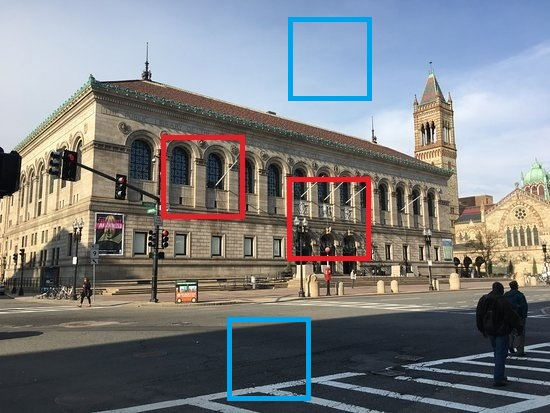
\includegraphics[width=0.41\textwidth]{img/library}
\\[0.1cm]
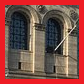
\includegraphics[width=0.1\textwidth]{img/library_1}

\includegraphics[width=0.1\textwidth]{img/library_2}

\includegraphics[width=0.1\textwidth]{img/library_3}

\includegraphics[width=0.1\textwidth]{img/library_4}
\caption{An example of salient regions and non-salient regions of an image.}
\label{fig:library}
\end{figure}

% too many details, may move to beginning of solution section
% Therefore, we aim to use the attribute of saliency to guide image/video localization. 
% To estimate how salient a region is, we reconsider the fact that non-salient regions are less discernible. 
% In other words, non-salient regions would be more common than salient ones in the database. We introduce the concept \textbf{saliency score} to measure how salient a region is. 
% An intuitive idea is to set saliency score of a region inversely proportional to the number of its similar regions in the database. 
% To evaluate how similar two regions are, we need to apply convolutional neural network (CNN), which has been widely used in the field of deep learning, to extract features from images. 

% In another hand, after estimating the saliency score of each region in an image. 
% We propose an attention-based model to guide the geo-localization system to pay more attention to salient regions when localizing an image. 
% Consequently, the model tends to be a joint model to both estimate saliency score of regions utilizing a matching model and optimize the matching model with the saliency score. 

% We evaluate our method on two video/image geo-localization datasets. 
% The experimental result on Boston dataset have shown that our method works well on event video frame geo-localization task. 
% We also evaluated it on the Tokyo Time Machine dataset~\cite{Arandjelovic16} in order to support the efficiency of our method.

The contributions of this paper are threefold. 
\begin{enumerate}
\item We formulate the event video localization task as a joint saliency detection and matching problem. 
Such formulation distinguishs between meaningful matching and meaningless matching adaptively to district domain, preserves the interdependency between saliency and matching and enhances system explainability.  
\item We propose a self-paced learning styled solution for the joint model, which starts from easy saliency detection and matching cases and gradually move on to hard saliency detection and matching cases. 
% \item We demonstrate that saliency is an effective attribute to guide image/video localization. 
% \item We propose a method which can joint estimate the saliency score of image regions and geo-localize an image or a video.
% \item Our method is helpful for real world event related video geo-localization and it is efficient to solve cross-domain matching problems.
\end{enumerate}

% section arrangement
The rest of the paper is organized as follows. 
Section~\ref{sec:related} introduces related work. 
Section~\ref{sec:problem} formalizes the problem for the video event localization task. 
Section~\ref{sec:solution} gives the solution to the problem. 
Section~\ref{sec:expr} presents the experiment results. 
Section~\ref{sec:conclusion} draws some conclusions. 
